\documentclass{article}

\usepackage[]{mathtools} 
\usepackage[]{amssymb} 
\usepackage[]{microtype} 
\usepackage[]{enumerate} 

\usepackage[]{palatino} 
\usepackage[]{eulervm} 

\usepackage[]{amsthm} 
\usepackage[]{thmtools} 
\usepackage[usenames, dvipsnames, svgnames, table]{xcolor} 
\usepackage[]{minted} 
\usepackage[]{hyperref} 
\usepackage[capitalize, noabbrev]{cleveref} 

\renewcommand{\S}{\mathbb{S}}
\newcommand{\B}{\mathcal{B}}
\newcommand{\R}{\boldsymbol{R}}
\newcommand{\rrho}{\boldsymbol{\rho}}
\newcommand{\aalpha}{\boldsymbol{\alpha}}

\let\oldemph\emph
\renewcommand{\emph}[1]{\textcolor{Maroon}{\oldemph{#1}}}

\declaretheoremstyle[
    headfont = \color{Maroon}\normalfont\bfseries,
    mdframed = {
        linecolor = Gray,
        backgroundcolor = Gray!10
    }
]{theorem}
\declaretheorem[
    style=theorem,
    name=Theorem,
    numbered=no,
]{theorem}
\declaretheorem[
    style=theorem,
    name=Recall,
    numbered=no,
]{recall}
\declaretheorem[
    style=theorem,
    name=Lemma,
    numbered=no,
]{lemma}
\title{\textsc{Assignment 3 \\
       MATINF4170 \\
       Spline Methods}
}
\author{Ivar Haugal{\o}kken Stangeby}

\begin{document}
    \maketitle 

    \section*{Exercise 3.1}
    
    In this exercise we wish to show the linear independence of two cubic
    B-splines on the knot vector $\hat{t} \coloneqq (0, 0, 1, 3, 4, 5)$ over
    the interval $[1, 3)$. Using the knot dependencies, these two B-splines are
    \begin{align*}
        \hat{B}_{1, 3}(x \mid 0, 0, 1, 3, 4), && \hat{B}_{2, 3}(x \mid 0, 1, 3,
        4, 5).
    \end{align*}
    In order to show the linear independence, we wish to apply Theorem 3.9,
    restated here:
    
    \begin{theorem}[3.9]
        Suppose that $t$ is a $p + 1$-extended knot vector. Then the B-splines
        in $\S_{p, t}$ are linearly independent on the interval $[t_{p+1},
        t_{n+1})$.
    \end{theorem}
    
    Note that the vector $\hat{t}$ is \emph{not} $p+1$-extended, so we
    introduce the new knot vector $t \coloneqq (0, 0, 0, 1, 3, 4, 5, 5)$.  We
    now have enough knots to define four cubic B-splines, and these are
    \begin{align*}
        &B_{1, 3}(x \mid 0, 0, 0, 1, 3), & &B_{2, 3}(x \mid 0, 0, 1, 3, 4), \\
        &B_{3, 3}(x \mid 0, 1, 3, 4, 5), & &B_{4, 3}(x \mid 1, 3, 4, 5, 5).
    \end{align*}
    By the above theorem, we now know that the B-splines $B_{i, 3, t}$ for $i =
    1, \ldots, 4$ are linearly independent on the interval $[t_{4}, t_{5}) =
    [1, 3)$.  By examining the knot dependencies, we see that $B_{2, 3} =
    \hat{B}_{1, 3}$ and $B_{3, 3} = \hat{B}_{2, 3}$. Hence, the two B-splines
    on the coarse knot vector are linearly independent on the interval $[1,
    3)$.
    
    \section*{Exercise 4.5}
    
    In this exercise, we wish to prove Lemma 4.2 in generality:
    \begin{lemma}[4.2]
        Let $p$ be a positive integer and let $\tau$ be a knot vector with at
        least $p+2$ knots. If $t$ is a knot vector containing $\tau$ as a
        subsequence, then $\S_{p, \tau} \subseteq \S_{p, t}$.
    \end{lemma}
    The requirement that $\tau$ contains at least $p + 2$ knots ensures that we
    have at least one B-spline in the coarse spline space.  We want to apply
    Curry-Schoenberg, however our knot vectors are not $p+1$-regular. Setting
    $a \coloneqq \min(t_1, \tau_1) - 1$ and $b \coloneqq \max(t_n, \tau_m) + 1$
    we can introduce the augmented knot vectors
    \begin{align*}
        t' &\coloneqq (\overbrace{a, \ldots, a}^{p+1}, t_1, \ldots, t_n\,\,,
        \overbrace{b, \ldots, b}^{p+1}), \\ \tau' &\coloneqq (\underbrace{a,
    \ldots, a}_{p+1}, \tau_1, \ldots, \tau_m, \underbrace{b, \ldots, b}_{p+1}).
    \end{align*}
    By Curry-Schoenberg, we have the following inclusions:
    \begin{equation}
        \notag
        \S_{p, \tau} \subseteq \S_{p, \tau'} = \S_p^{r_{\tau'}}(\Delta_{\tau'}) \subseteq
        \S_p^{r_{t'}}(\Delta_{t'}) = \S_{p, t'} \supseteq \S_{p, t}, 
    \end{equation}
    where $r_{\tau'}$ and $r_{t'}$ are the continuity requirements imposed by
    $\tau'$ and $t'$ respectively.  This implies that any $f \in \S_{p, \tau}$
    also lies in $\S_{p, t'}$. It now remains to show that $f$ also must lie in
    $\S_{p, t}$.

    By construction, the first $p+1$, and the last $p+1$ spline coefficients of
    a spline $f$ in $\S_{p, \tau}$ with respect to the knot vector $\tau'$ are
    zero. Consequently, the first $p+1$ and last $p+1$ spline coefficients of
    $f$ with respect to the knot vector $t'$ are zero. This means, that only
    the B-splines originally defined on the refined knot vector $t$ contributes
    to the spline $f$. Hence, $f \in \S_{p, t'}$.
    
    \section*{Exercise 4.6}
    
    In this exercise, we want to show that Theorem 4.6 holds in the general
    case, where $\tau$ and $t$ not necessarily are $p+1$ regular. For this, we
    recall the following:
    \begin{recall}
        These results will be needed:     
        \begin{enumerate}[i)]
            \item $\R_1(x_1)\cdots\R_p(x_p)\rrho_p(y) = (y - x_1)\cdots(y-x_p)$.
            \item If $\tau \subseteq t$ are two $p+1$ regular knot vectors with common end knots, then
                \begin{align*}
                    \rho_{i, p, t}(y) = \aalpha_p(i)\rrho_{p, \tau}(y) && b_i = \aalpha_p(i)c_p.
                \end{align*}
            \item The dual polynomials in $\rrho_{p, \tau}(y)$ are linearily
                independent.
        \end{enumerate} 
    \end{recall}
    Let $\tau'$ and $t'$ be the augmented knot vectors as defined in Exercise
    4.5. For $p = 0$, if $\tau'_\mu \leq t'_i < \tau'_{\mu+1}$, then
    $\alpha_{p}(i) = 1$. If $p > 0$, then we know that
    \begin{equation}
        \notag
        \R_1(x_1)\cdots\R_p(x_p)\rrho_{p, \tau'}(y) = (y - x_1)\cdots(y-x_p)
    \end{equation}
    and letting $x_j = t'_{i+j}$ yields
    \begin{equation}
        \notag
        \R_1(t'_{i+1}) \cdots \R_p(t'_{i+p})\rrho_{p, \tau'}(y) = (y -
        t'_{j+1}) \cdots (y - t'_{j+p}) = \rho_{i, p, t'}(y).
    \end{equation}
    As we recalled, we can write $\rho_{i, p, t'}(y) = \aalpha_p(i)\rrho_{p,
    \tau}$, so this reduces to
    \begin{equation}
        \notag
        \R_1(t'_{i+1}) \cdots \R_p(t'_{i+p})\rrho_{p, \tau'}(y)
        =\aalpha_p(i)\rrho_{p, \tau'}(y).
    \end{equation}
    By the linear independence of the dual polynomials, this means that
    \begin{equation}
        \notag
        \R_1(t'_{i+1}) \cdots \R_p(t'_{i+p})) = \aalpha_p(i).
    \end{equation}
    This has proven the result for the $p+1$ regular vectors $\tau'$ and $t'$.
    Assume we have $n$ B-splines in $\S_{p, \tau}$ and $m$ B-splines in $\S_{p,
    t}$. In our augmented knot vectors, as the first $p+1$ and last $p+1$ knots
    are equal, the first $p+1$ and last $p+1$ rows of the knot insertion matrix
    is zero. For each non-zero row, that is rows $i = p+2, \ldots, m+p+1$, only
    columns $j = p+1, \ldots, n+p+1$ correspond to the old coarse B-splines.
    Hence, we can consider the submatrix obtained by dropping the $p+1$ first
    and last rows and columns.

    \section*{Exercise 4.7}
    In this exercise, we show that the $p+1$ \emph{discrete B-splines} of
    degree $p$ sums to one, provided that $\tau$ and $t$ are $p+1$ regular and
    $\tau \subseteq t$ with knots agreeing at the end.

    \begin{recall}
        The discrete B-splines satisfy the following recurrence relation:
        \begin{equation}
            \notag
            \alpha_{j, p}(i) = \frac{t_{i+p} - \tau_j}{\tau_{j+p} - \tau_j}
            \alpha_{j, p-1}(i) + \frac{\tau_{j+p+1}-t_{i+p}}{\tau_{j+1+p}
            -\tau_{j+1}}\alpha_{j+1, p-1}(i),
        \end{equation}
        where $\alpha_{j, 0}(i) = B_{j, 0}(t_i)$.
    \end{recall}
    We proceed by induction.
    \paragraph{Base case:} The base case consists of $p = 0$ where we have
    \begin{equation}
        \notag
        \sum_{j} \alpha_{j, 0}(i) = \sum_{j} B_{j, 0}(i) = 1,
    \end{equation}
    as the B-splines sum to 1.
    
    \paragraph{Induction step:}
    We assume for the sake of induction that the claim holds for degree $p-1$,
    and wish to show that it also holds for degree $p$. We know that
    $\alpha_{j, p}(i) = 0$ for $j < \mu - p$ and $j > \mu$, so we can discard
    the discrete B-splines not contributing to the sum. We then have that
    \begin{equation}
        \notag
        \sum_{j = \mu - p}^{\mu} \alpha_{j, p}(i) = \sum_{j= \mu - p}^{\mu}
        \frac{t_{i+p} - \tau_j}{\tau_{j+p} - \tau_j} \alpha_{j, p-1}(i) +
        \sum_{j=\mu - p}^{\mu} \frac{\tau_{j+p+1}-t_{i+p}}{\tau_{j+1+p}
        -\tau_{j+1}}\alpha_{j+1, p-1}(i),
    \end{equation}
    by the recurrence relation. Now, since we are working with discrete
    B-splines of one less degree, we have that for $j < \mu - p + 1$ and $j >
    \mu$ the discrete B-splines $\alpha_{j, p-1}(i) = 0$. We can therefore
    discard $\alpha_{\mu - p, p-1}(i)$ and $\alpha_{\mu + 1, p-1}(i)$ as they
    are both zero. By a change of summation index, we end up with the following:
    \begin{equation}
        \notag
        \sum_{j=\mu - p}^\mu \alpha_{j, p}(i) = \sum^{\mu}_{j=\mu - p + 1}
        \frac{\tau_{j+p} - \tau_{j}}{\tau_{j+p} - \tau_{j}} \alpha_{j, p-1}(i) =
        1,
    \end{equation}
    where the last equality follows by the induction hypothesis. This closes
    the induction.
    
    \section*{Exercise 4.8}
    In this exercise, we implement the \emph{Oslo algorithm} for computing knot
    insertion matrices and the refinement of coefficient vectors. The Oslo
    algorithms have a striking resemblance to the spline evaluation algorithms,
    where the spline is ``evaluated'' at the fine knots.

    We first implement a routine for inserting midpoints in the non-trivial
    knot intervals in a given $p+1$-extended knot vector for a given spline
    degree $p$. A \textsc{Python} implementation is given in
    \cref{lst:midpoints}. This method will be used for repeated refinenement of
    a knot vector, to illustrate that the control polygon of a spline converges
    under repeated knot insertion.
    
    The Oslo algorithm for computing the coefficients of a coarse B-spline as a
    linear combination of finer B-splines is implemented in \textsc{Python} as
    shown in \cref{lst:oslo}.

    The algorithm was used to examine the convergence of the control polygon to
    the spline under repeated knot insertion. Here we simply insert midpoints
    where possible. The results are given in
    \cref{fig:pictures/example_1,fig:pictures/example_2}.
    \begin{figure}[htpb]
        \centering
        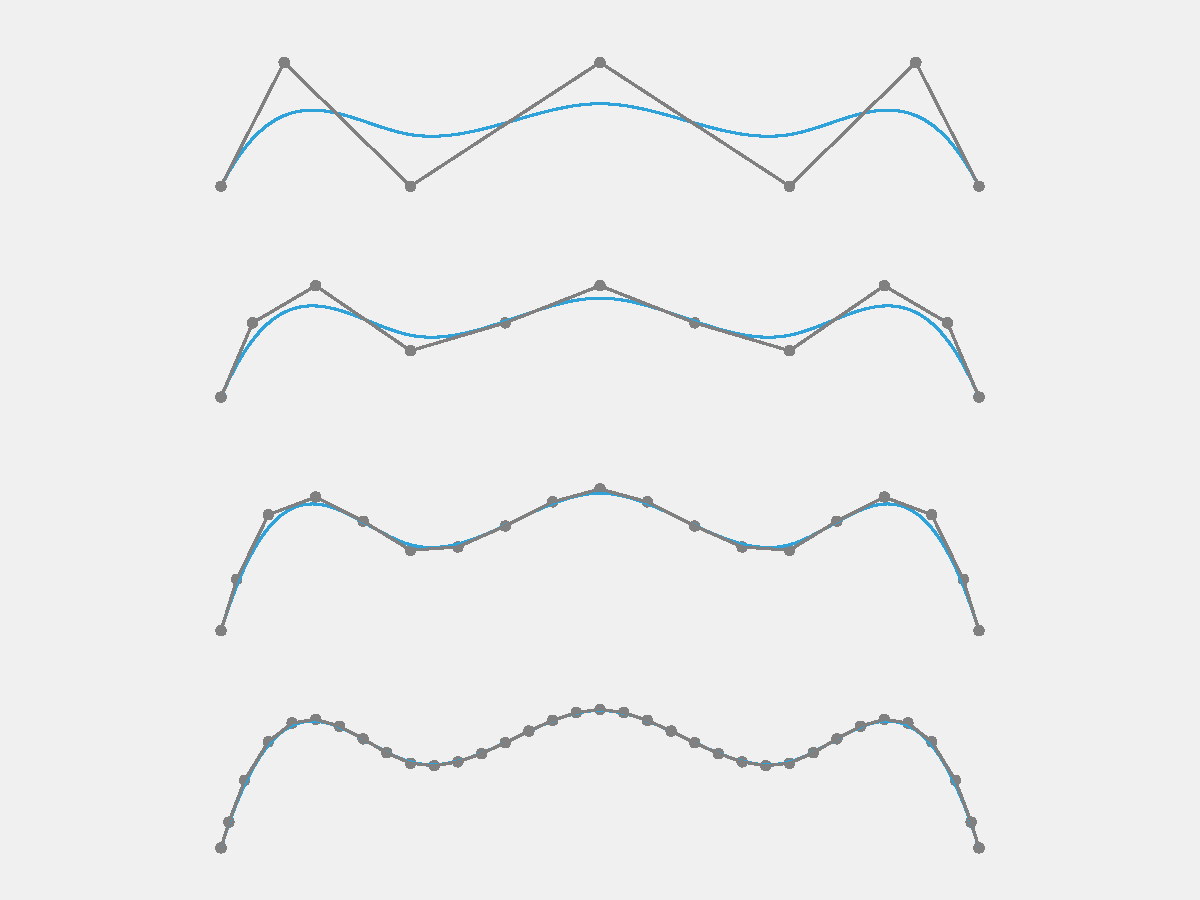
\includegraphics[width=0.8\linewidth]{pictures/example_1.pdf}
        \caption{
            A cubic spline over the knot vector $t = [0, 0, 0, 0, 1, 2, 3, 4,
            4, 4, 4]$ with corresponding spline coefficients $c = [-1, 1, -1,
            1, -1, 1, -1]$. The top image is the control polygon with no
            refinements of the knot vector. Then, the three following splines
            are with one, two and three midpoint refinements respectively.
        }
        \label{fig:pictures/example_1} 
    \end{figure}
\begin{figure}[htpb]
        \centering
        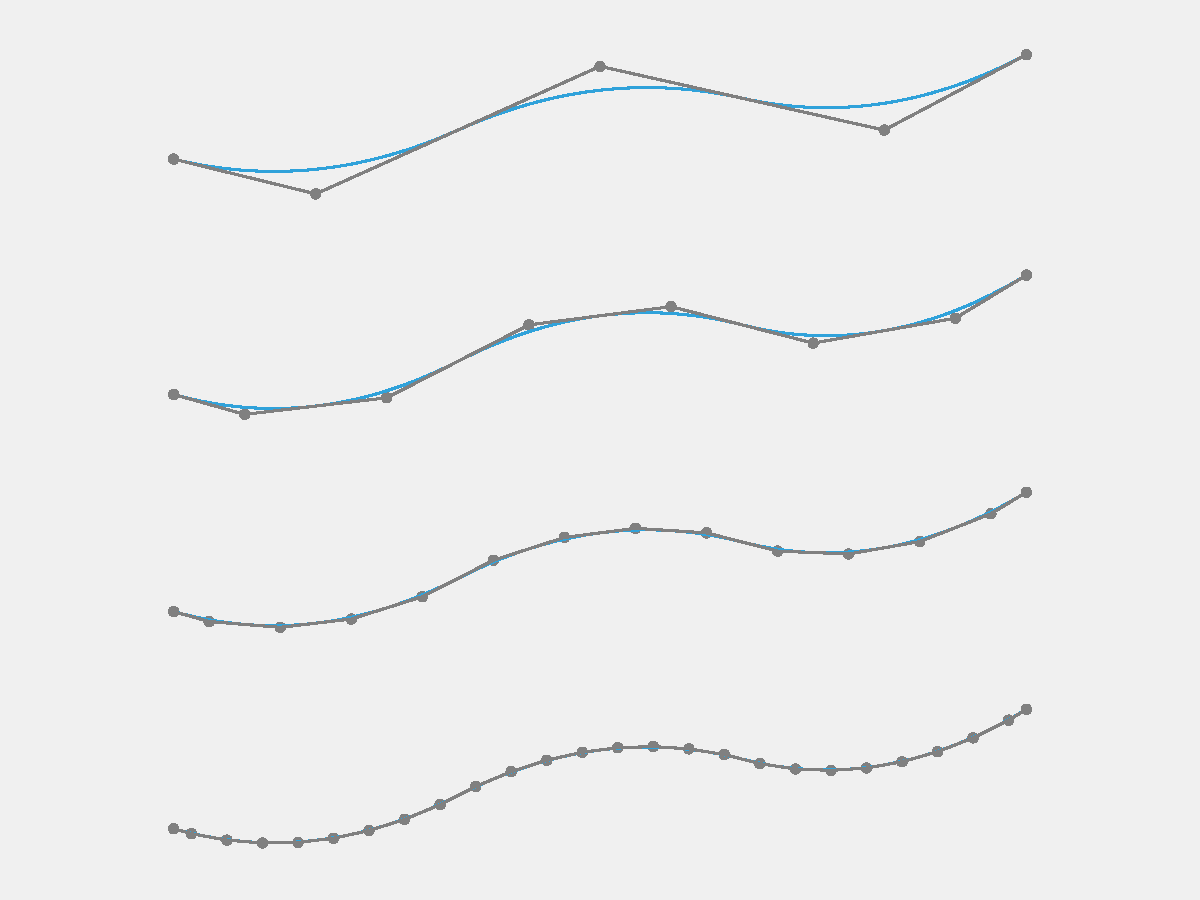
\includegraphics[width=0.8\linewidth]{pictures/example_2.pdf}
        \caption{
            A quadratic spline over the knot vector $t = [0, 0, 0, 1, 2, 3, 3,
            3]$ with corresponding spline coefficients $c = [-3, -6, 5, -0.5,
            6]$. The top image is the control polygon with no refinements of
            the knot vector. Then, the three following splines are with one,
            two and three midpoint refinements respectively.
        }
        \label{fig:pictures/example_2} 
    \end{figure}

    \begin{listing}[htbp]
    \begin{minted}{python}
def insert_midpoints(x, p):
    """
    Routine for inserting n - 1 midpoints in a p+1 
    extended knot vector, using numpy vector operations.
    :param x: the knot vector x
    :param p: the spline degree p
    :return: knot vector with inserted midpoints
    """
    midpoints = (x[p:-p - 1] + x[p + 1:-p]) / 2
    m = len(midpoints)
    new_array = np.zeros(len(x) + m, dtype=np.float64)

    new_array[:p + 1] = x[:p + 1]
    new_array[-p - 1:] = x[-p - 1]
    new_array[p + 1:p + 2 * m:2] = midpoints
    new_array[p + 2:p + 2 * m - 1:2] = x[p + 1:-p - 1]

    return new_array
    \end{minted}
    \caption{Inserts midpoints in the non-trivial intervals of a $p+1$ extended
    knot vector. The interior knots are supposed to be strictly increasing.}
    \label{lst:midpoints}
\end{listing}

\begin{listing}[htbp]
    \begin{minted}{python}
def algorithm_4_10(p, tau, t, c):
    """
    Computes the spline coefficients representing a coarse 
    spline in a finer spline space.
    :param p: The spline degree
    :param tau: The coarse knot vector
    :param t: The fine knot vector
    :param c: The set of coarse spline coefficients
    :return: The set of fine spline coefficients
    """

    m = len(t) - (p + 1)
    n = len(tau) - (p + 1)
    c = np.array(c, dtype=np.float64)
    t = np.array(t, dtype=np.float64)
    tau = np.array(tau, dtype=np.float64)
    b = np.zeros(m)

    for i in range(m):
        mu = index(t[i], tau)
        if p == 0:
            b[i] = c[mu]
        else:
            C = c[mu - p:mu + 1]
            for j in range(0, p):
                k = p - j
                tau1 = tau[mu - k + 1:mu + 1]
                tau2 = tau[mu + 1:mu + k + 1]
                omega = np.divide(
                    (t[i + k] - tau1), (tau2 - tau1),
                    out=np.zeros_like(tau1),
                    where=((tau2 - tau1) != 0))
                C = (1 - omega) * C[:-1] + omega * C[1:]
            b[i] = C
    return b
    \end{minted}
    \caption{The Oslo algorithm implemented in \textsc{Python}. Given a coarse
    knot vector, we can refine the corresponding spline space and represent the
coarse splines as linear combinations of the finer B-splines.}
    \label{lst:oslo} 
\end{listing}
    
    \section*{Exercise 4.10}
    
    In this exercise, we find the trivariate blossoms of some given
    polynomials.

    \begin{recall}
        The $p$-variate \emph{blossom} of $g \in \Pi_p$ satisfies:
        \begin{enumerate}[i)]
            \item $\B[g](x_1, \ldots, x_p) = \B[g](x_{\sigma(1)}, \ldots,
                x_{\sigma(p)})$ where $\sigma \colon \{1, \ldots, p\} \to \{1,
                \ldots, p\}$ is a permutation;
            \item $\B[g](\ldots, \alpha x + \beta y, \ldots) = \alpha
                    \B[g](\ldots, x, \ldots) + \beta\B[g](\ldots, y, \ldots)$
                    when $\alpha + \beta = 1$;
                \item $\B[g](x, \ldots, x) = g(x).$
        \end{enumerate}
    \end{recall}
    It then follows that the blossoms of the following polynomials are:
    \begin{enumerate}[a)]
        \item $\B[x^3] = x_1 x_2 x_3$;
        \item $\B[1] = 1$;
        \item $\B[2x + x^2 - 4x^3] = 2 (x_1 + x_2 + x_3)/3 + (x_1x_2 + x_1x_3 +
            x_2x_3)/3 - 4x_1x_2x_3$;
        \item $\B[0] = 0$;
        \item $\B[(x-a)^2] = (x_1x_2 + x_1x_3 + x_2x_3) / 3 - 2a (x_1 + x_2 +
            x_3) / 3 + a^2$.
    \end{enumerate}
    
\end{document}
